\documentclass[10pt, letterpaper]{exam}
\usepackage{graphicx}
%\usepackage[a4paper, total={7in, 11in}]{geometry}
\usepackage[letterpaper, total={7in, 10in}]{geometry}
\usepackage[normalem]{ulem}
\usepackage{amsmath}
\renewcommand\ULthickness{1.0pt}   
\setlength\ULdepth{1.3ex}

\begin{document}
	\noindent
	\begin{minipage}[l]{0.1\textwidth}
		\noindent
		
\includegraphics[width=2.8\textwidth]{ESCUDO.png}
	\end{minipage}
\hfill
\begin{minipage}[c]{0.8\textwidth}
	\begin{center}
		{\large  Departamento de Ingeniería civil y Agrícola\par
		\large	Facultad de Ingeniería	\par
	% \large \textbf{Taller propiedades de los fluidos}	\par
    \large \textbf{Quiz Laboratorio No. 2: Resalto hidr\'aulico}	\par
} Prof. Luis Alejandro Morales (Ph.D) 
	\end{center}
\end{minipage}
\par
\vspace{0.2in}
\noindent
    \uline{Mecánica de fluidos [2015966]	\hfill 2023-I	}
\par 
\vspace{0.15in}
\noindent

%%%%%%%%%%%%%%%%%%%%%%%%%%%%%
En un canal de laboratorio horizontal y rectangular de ancho $b=3\ m$ se observa un resalto hidr\'aulico  cuyas profundidades aguas arriba y aguas abajo  son $y_1 = 0.6\ m$ y $y_2 = 1.5\ m$, respectivamente. Realizar lo siguiente:

%En el laboratorio de hidr\'aulica de la Universidad Nacional de Colombia, estudiantes del curso de Mec\'anica de Fluidos realizaron un laboratorio sobre conservaci\'on de la cantidad de movimiento en donde generaron un resalto hidr\'aulico en un canal horizontal de ancho $b = $ 31 $cm$ que transporta agua con $\rho =$ 1000 $kg\ m^{-3}$. Los estudiantes tomaron la profundidad de la l\'amina de agua aguas arriba de la compuerta $y_0 = $ 60 $cm$ y aguas abajo de la misma al inicio del resalto hidr\'aulico $y_1 = $ 7 $cm$ (ver figura~\ref{f1}).

%De acuerdo con la informaci\'on tomada, ellos deberan realizar lo siguiente:
\begin{enumerate}
    \item Calcular el caudal que transporte el canal.
    %\item Calcular la altura conjugada $y_2$ aguas abajo del resaldo hidr\'aulico
    %\item Calcular las alturas conjugadas en el resalto $y_1$  (aguas arriba) y $y_2$ (aguas abajo).
    \item Calcular el n\'umero de Froude aguas arriba y aguas abajo del resalto.
    \item Calcular las p\'erdidas de energ\'ia en el resalto.
    \item Para diferentes valores de $y$, incluyendo $y_1$, $y_c$ (profundidad cr\'itica) y $y_2$, esquematizar la curva de fuerza espec\'ifica.
\end{enumerate}

Ayuda:
\vspace{-0.5cm}
\begin{equation*} 
\begin{split}
& F_s = A \bar{h} + \frac{Q^2}{gA} \\
& \frac{y_2}{y_1} = \frac{1}{2}\left[ \sqrt{1+8F_{R_1}^2 } -1 \right]
\end{split}
\end{equation*}



%\begin{figure}[h]
%    \centering
%    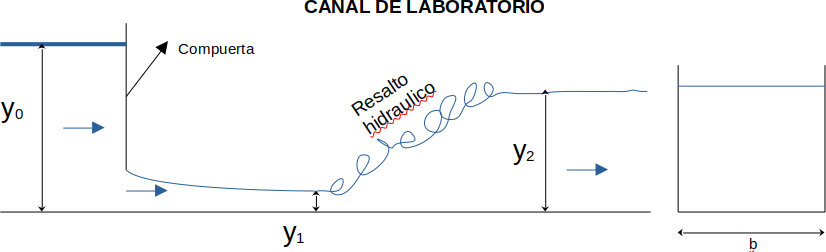
\includegraphics[width=\textwidth]{canalLab}
%    \label{f1}
%\end{figure}
\end{document}



